%% LaTeX-Beamer template for KIT design
%% by Erik Burger, Christian Hammer
%% title picture by Klaus Krogmann
%%
%% version 2.1
%%
%% mostly compatible to KIT corporate design v2.0
%% http://intranet.kit.edu/gestaltungsrichtlinien.php
%%
%% Problems, bugs and comments to
%% burger@kit.edu

\documentclass[18pt]{beamer}
\usepackage[utf8]{inputenc}
%% SLIDE FORMAT

% use 'beamerthemekit' for standard 4:3 ratio
% for widescreen slides (16:9), use 'beamerthemekitwide'

\usepackage{templates/beamerthemekit}
% \usepackage{templates/beamerthemekitwide}

%% TITLE PICTURE

% if a custom picture is to be used on the title page, copy it into the 'logos'
% directory, in the line below, replace 'mypicture' with the 
% filename (without extension) and uncomment the following line
% (picture proportions: 63 : 20 for standard, 169 : 40 for wide
% *.eps format if you use latex+dvips+ps2pdf, 
% *.jpg/*.png/*.pdf if you use pdflatex)

%\titleimage{mypicture}

%% TITLE LOGO

% for a custom logo on the front page, copy your file into the 'logos'
% directory, insert the filename in the line below and uncomment it

%\titlelogo{mylogo}

% (*.eps format if you use latex+dvips+ps2pdf,
% *.jpg/*.png/*.pdf if you use pdflatex)

%% TikZ INTEGRATION

% use these packages for PCM symbols and UML classes
% \usepackage{templates/tikzkit}
% \usepackage{templates/tikzuml}

% the presentation starts here

\title[Geometrie 2]{Geometrie 2 - ICPC Praktikum SS14}


\institute{Tobias Hornberger $\cdot$ Paul Jungeblut $\cdot$ Enja Stein $\cdot$ Lena Winter}

\begin{document}

% change the following line to "ngerman" for German style date and logos
\selectlanguage{ngerman}

%title page
\begin{frame}
\titlepage
\end{frame}

\section{Konvexe Hülle}
	\subsection{Problemstellung}
		\begin{frame}{Problemstellung: Konvexe Hülle}
			\begin{box}
			 Gegeben sei eine Menge M von Punkten in der Ebene. Die konvexe Hülle von M ist die kleinste konvexe Menge, in der M enthalten ist.
			\end{box}
			\begin{figure}
				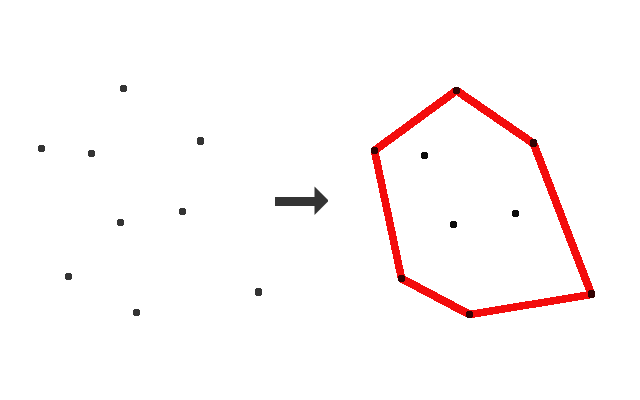
\includegraphics[width=8cm]{logos/konhu.png}\\
			\end{figure}
		\end{frame}
	
	\subsection{Graham Scan}
		\begin{frame}{Idee: Graham Scan}
	
		\end{frame}
	
		\begin{frame}{Pseudocode}
	
		\end{frame}

\section{Sweepline}

	\subsection{Problemstellung}
		\begin{frame}{Problemstellung: Linienschnitt}
		\end{frame}
	
	\subsection{Sweepline}
		\begin{frame}{Idee: Sweepline}
	
		\end{frame}
	
		\begin{frame}{Pseudocode}
	
		\end{frame}
	
\section{Closed Pair}

	\subsection{Problemstellung}
		\begin{frame}{Problemstellung: Closed Pair}
			\textbf{Geben:} n Punkte auf einer Ebene \\
			\textbf{Gesucht:} die beiden am nähesten zusammenliegenden Punkte\\
			
		\end{frame}
	
	\subsection{Divide and Conquer}
		\begin{frame}{Idee: Divide and Conquer}
	
		\end{frame}
	
		\begin{frame}{Pseudocode}
	
		\end{frame}
	

\end{document}
